%\documentclass[wcp,gray]{jmlr} % test grayscale version
\documentclass[10pt]{jmlr}% former name JMLR W\&CP
%\documentclass[pmlr]{jmlr}% new name PMLR (Proceedings of Machine Learning)

 % The following packages will be automatically loaded:
 % amsmath, amssymb, natbib, graphicx, url, algorithm2e
 \usepackage{amsmath,amssymb,graphicx,url}
 \graphicspath{ {./Figures/} }

 %\usepackage{rotating}% for sideways figures and tables
\usepackage{longtable}% for long tables

 % The booktabs package is used by this sample document
 % (it provides \toprule, \midrule and \bottomrule).
 % Remove the next line if you don't require it.
\usepackage{booktabs}
 % The siunitx package is used by this sample document
 % to align numbers in a column by their decimal point.
 % Remove the next line if you don't require it.
\usepackage[load-configurations=version-1]{siunitx} % newer version
 %\usepackage{siunitx}

% Package to make table with multi rows and columns
\usepackage{multirow}
 
 % to do
\usepackage{xcolor}
\newcommand\todo[1]{\textcolor{red}{#1}}

 % change the arguments, as appropriate, in the following:
\jmlrvolume{}
\jmlryear{}
\jmlrworkshop{STA723 -- Case Study 1}
\jmlrproceedings{}{}


\usepackage[toc,page]{appendix}



% start article
% \titlebreak
% \footnote{}
% \textsf

\title[Modeling Price and Popularity of AirBnB listings in New-York]{Modeling Price and Popularity of AirBnB listings in New-York}	%\titletag{\thanks{XXX}} % leave empty?

 % Use \Name{Author Name} to specify the name.
 % If the surname contains spaces, enclose the surname
 % in braces, e.g. \Name{John {Smith Jones}} similarly
 % if the name has a "von" part, e.g \Name{Jane {de Winter}}.
 % If the first letter in the forenames is a diacritic
 % enclose the diacritic in braces, e.g. \Name{{\'E}louise Smith}

 % Authors with different addresses:
 
 \author[Jiang, Morsomme, Nwankwo]{Melody Jiang \and Raphael Morsomme \and Ezinne Nwankwo}
 \date{\today} % Date, can be changed to a custom date

 % Three or more authors with the same address:
 % \author{\Name{Author Name1} \Email{an1@sample.com}\\
 %  \Name{Author Name2} \Email{an2@sample.com}\\
 %  \Name{Author Name3} \Email{an3@sample.com}\\
 %  \addr Address}

 % Authors with different addresses:
 % \author{\Name{Author Name1} \Email{abc@sample.com}\\
 % \addr Address 1
 % \AND
 % \Name{Author Name2} \Email{xyz@sample.com}\\
 % \addr Address 2
 %}

% leave editor's section empty?
%\editor{Editor's name}
% \editors{List of editors' names}

\begin{document}

\maketitle

\begin{abstract}
This is abstract. 
\end{abstract}
\newpage
%%%%%%%%%%%%%%%%%%%%%%%%%%%%%%%%%%%%%%%%%%%%%%%%%%%%%%%%%%%%%
% INTRODUCTION
%%%%%%%%%%%%%%%%%%%%%%%%%%%%%%%%%%%%%%%%%%%%%%%%%%%%%%%%%%%%%
\section{Introduction}
\label{sec:intro}

This is introduction


%%%%%%%%%%%%%%%%%%%%%%%%%%%%%%%%%%%%%%%%%%%%%%%%%%%%%%%%%%%%%
% METHODS
%%%%%%%%%%%%%%%%%%%%%%%%%%%%%%%%%%%%%%%%%%%%%%%%%%%%%%%%%%%%%
\section{Methods}
\label{sec:method}

\subsection{Data}
\label{sec:data}
Here we describe data.

\subsection{Feature Engineering}
\label{sec:feature}
Here we describe feature engineering.



\subsection{Ordinal Logistic Regression Model}
Here is our model.


%%%%%%%%%%%%%%%%%%%%%%%%%%%%%%%%%%%%%%%%%%%%%%%%%%%%%%%%%%%%%
% RESULTS
%%%%%%%%%%%%%%%%%%%%%%%%%%%%%%%%%%%%%%%%%%%%%%%%%%%%%%%%%%%%%
\section{Results}
\label{sec:results}

%%%%%%%%%%%%%%%%%%%%%%%%%%%%%%%%% EDA
\subsection{EDA}

\figureref{fig:length_stay_density} shows the distribution of required minimum number of nights to book a listing. We observe that minimum number of nights is concetnrated at below 14 days and around 30 days. \figureref{fig:availability_density} displays the distribution of days that listings are available for booking in a year. We see that there are data concentrated at 0, which means these listings are not open for booking. Such observation would inform our data cleaning.

To address the quesstion of whether the type of listing (shared room, private room, entire home) vary across neighbourhoods, we performed a chi-square test and plotted the results in \figureref{fig:room_type}. The p-value of the chi-square test was less than $10^{-16}$, indicating that the type of listing does vary across neighbourhoods. In \figureref{fig:room_type}, the size of dots represents the absolute standardized residuals. The color represents the value of standardized residuals. We see that difference in room types is most pronounced in Manhattan and Queens. Manhattan has more entire home than expected and Queens has more private room than expected.

\figureref{fig:map_eda} shows a spatial map of  of listings, metro stations, and attractions. Black dots represent metro stations, gree dots attractions, blue dots listings priced at bottom 80\%, and red dots are listings priced at top 20\%. We observe that listings priced at top 20\% distribute close to metro stations. This observation motivates us to include spatial in formation of metro stations as explanatory variables.



%%%%%%%%%%%%%%%%%%%%%%%%%%%%%%%%% MAIN FINDINGS
\subsection{Main Findings}
Main findings.

%%%%%%%%%%%%%%%%%%%%%%%%%%%%%%%%% SENSITIVITY ANALYSIS
\subsection{Sensitivity Analysis}
Sensitivity analysis.

\section{Conclusions and further discussion}
\label{sec:conclusion}
Conclusion and further discussions.


\newpage %%%% Ensures that Bibliography stays in one separate page.
\begin{thebibliography}{99} % Beamer does not support BibTeX so references must be inserted manually as below
	
	
	
\end{thebibliography}


%%%%%%%%%%%%%%%%%%%%%%%%%%%%%%%%%%%%%%%%%%%%%%%%%%%%%%%%%%%%%
% APPENDIX
%%%%%%%%%%%%%%%%%%%%%%%%%%%%%%%%%%%%%%%%%%%%%%%%%%%%%%%%%%%%%
\newpage
\appendix

%%%%%%%%%%%%%%%%%%%%%%%%%%%%%%%%% BOX COX
\section{Figures and Tables}
\label{appendix:fig}

\begin{figure}[htbp]
	\centering
	\caption{Distribution of minimum number of nights.}
	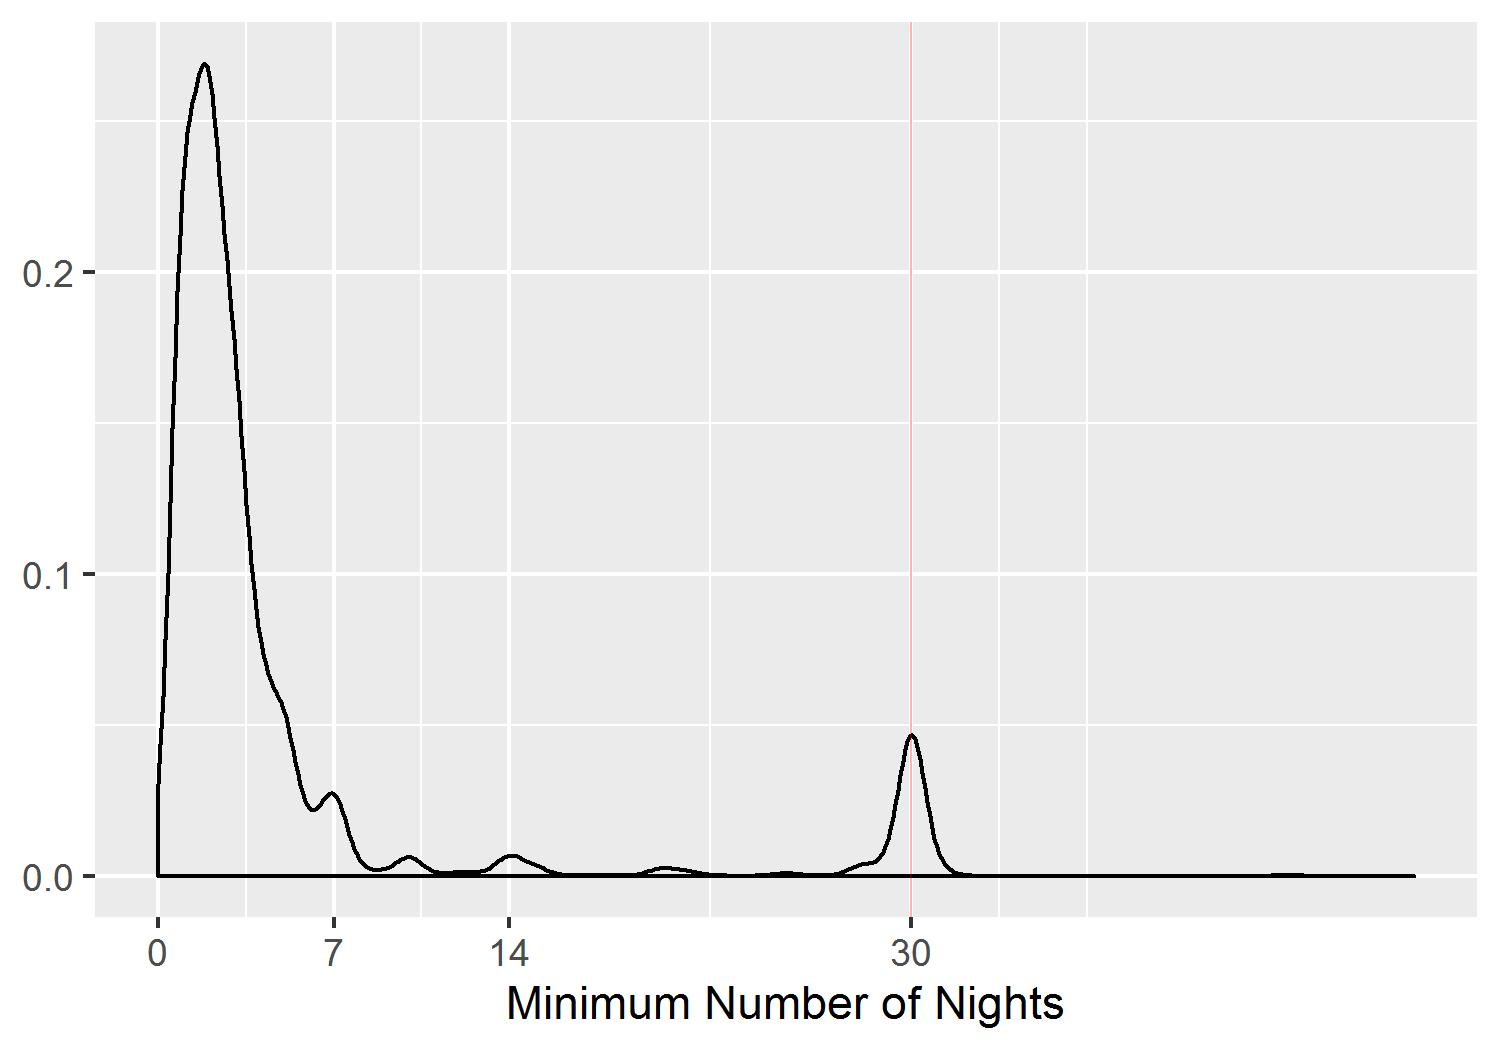
\includegraphics[width=0.5\linewidth]{length_stay_density.jpeg}
	\label{fig:length_stay_density}
\end{figure}

\begin{figure}[htbp]
	\centering
	\caption{Distribution of number of days available for booking.}
	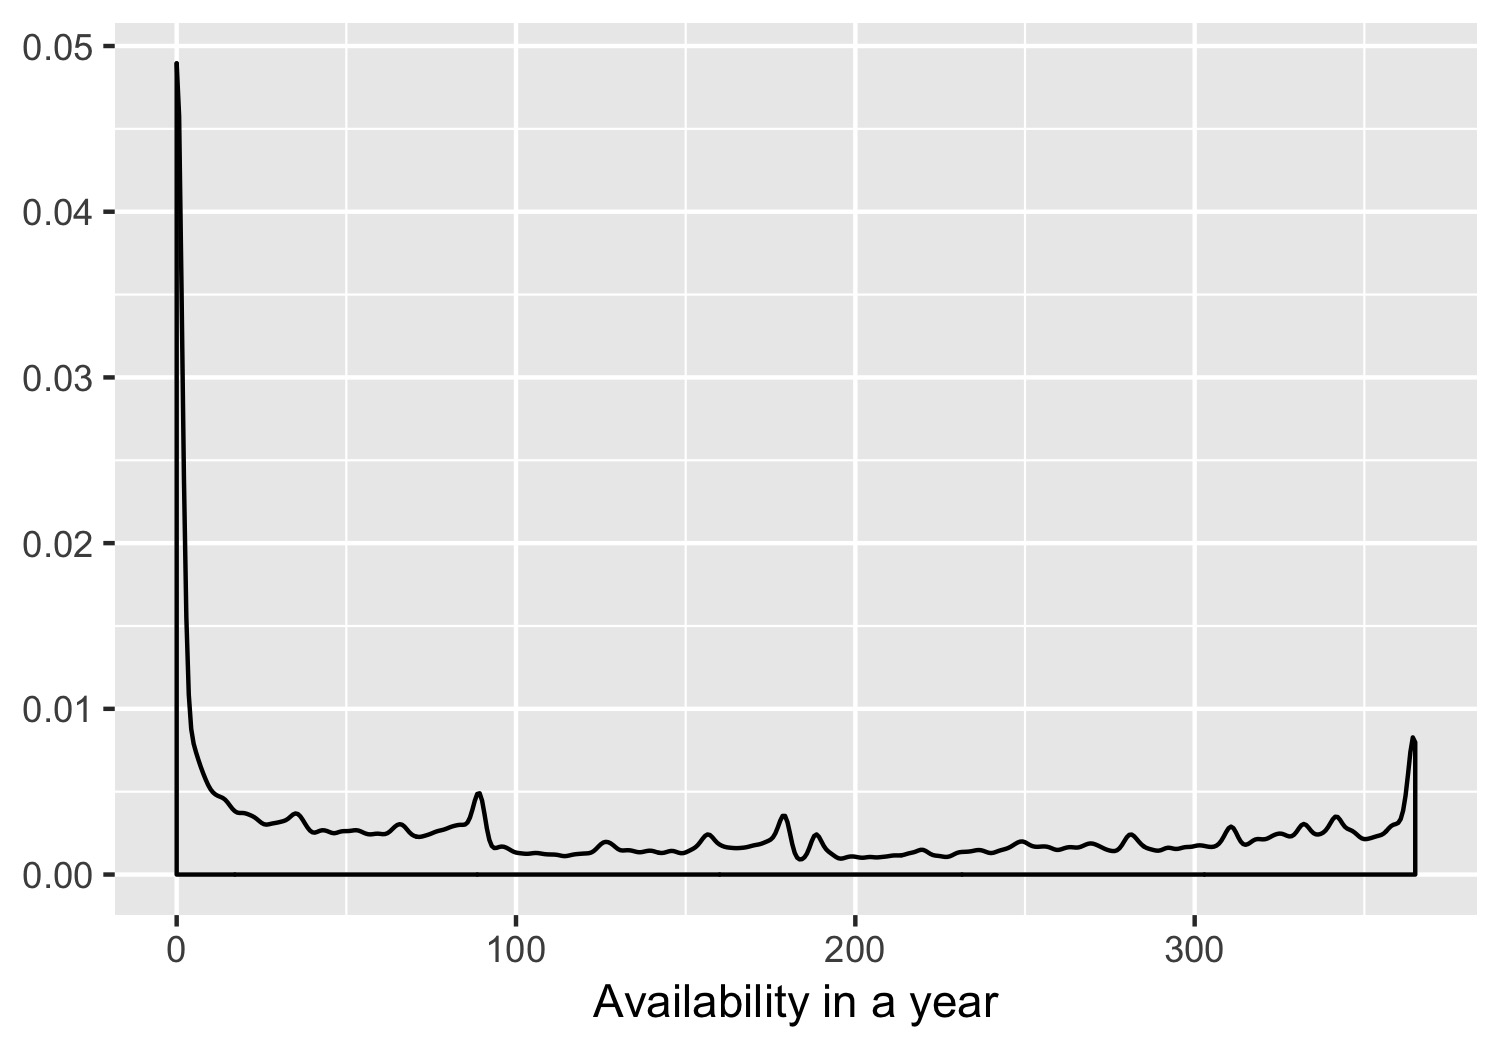
\includegraphics[width=0.5\linewidth]{availability_density.jpeg}
	\label{fig:availability_density}
\end{figure}

\begin{figure}[htbp]
	\centering
	\caption{Output from chi-squared test.}
	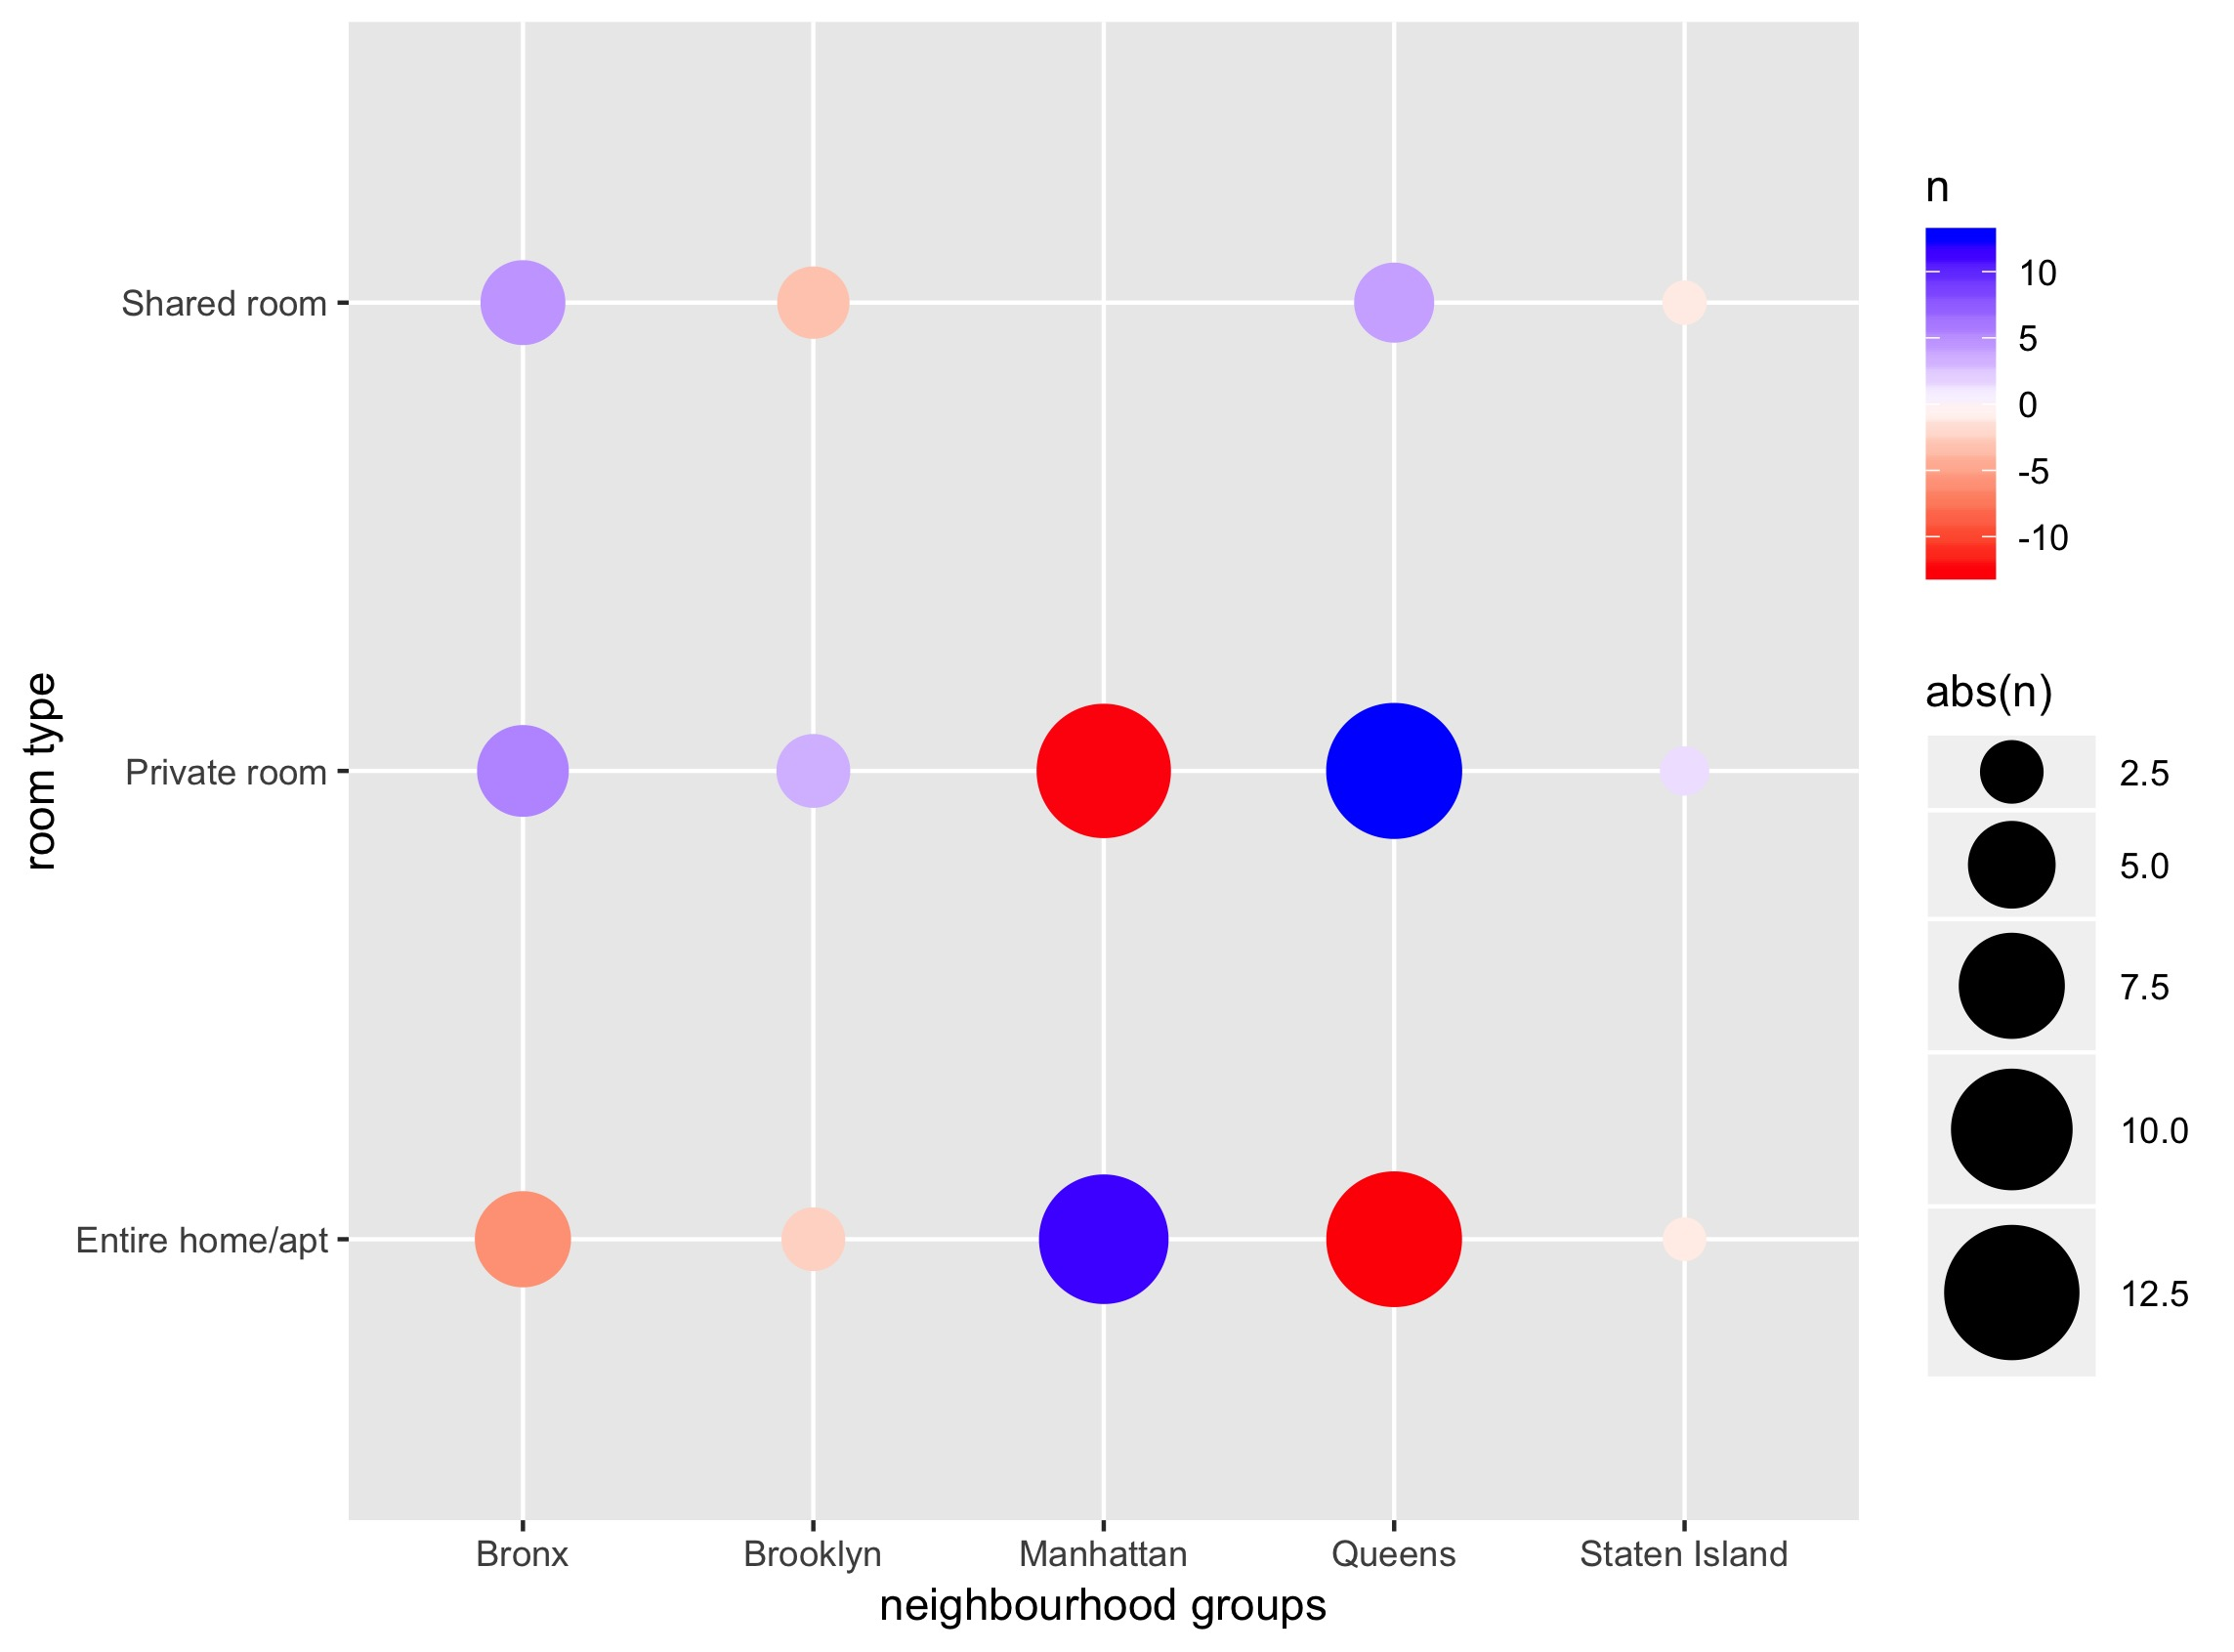
\includegraphics[width=0.5\linewidth]{room_type.jpeg}
	\label{fig:room_type}
\end{figure}

\begin{figure}[htbp]
	\centering
	\caption{Map of listings, metro stations, and attractions. Black dots are metro stations, gree dots are attractions, blue dots are listings priced at bottom 80\%, and red dots are listings priced at top 20\%}
	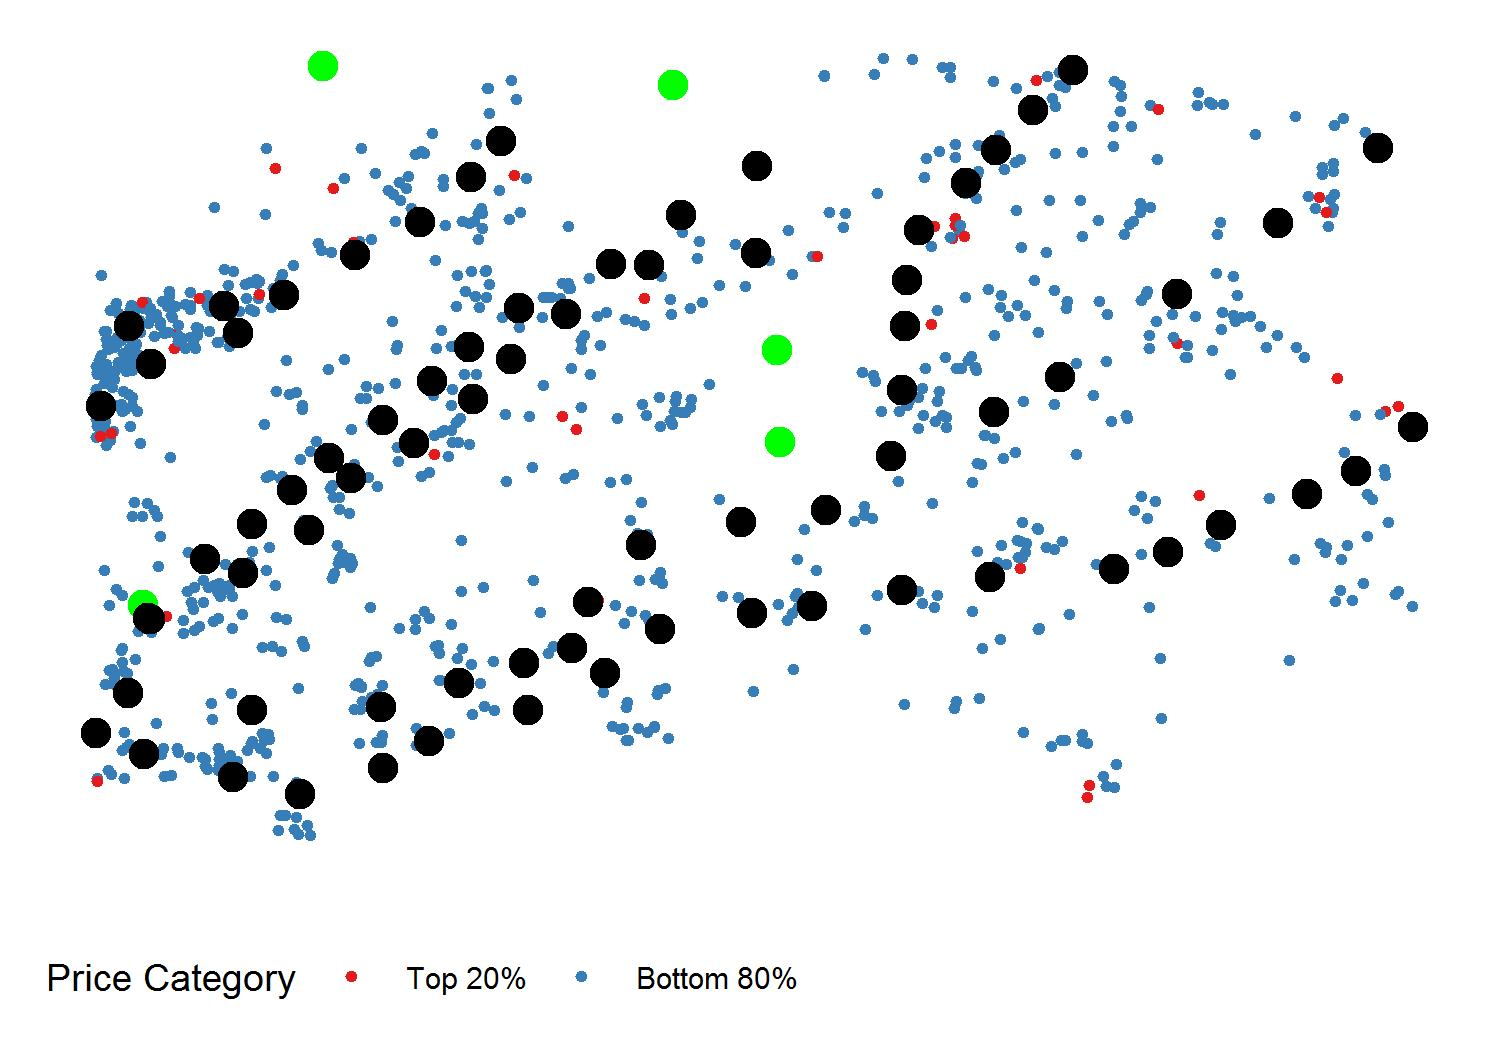
\includegraphics[width=0.5\linewidth]{map_eda.jpeg}
	\label{fig:map_eda}
\end{figure}

Figures here.

Tables here.

\newpage  % ensures that all figures remain together in appendix B

%%%%%%%%%%%%%%%%%%%%%%%%%%%%%%%%% MODEL CHECKING
\section{Model Checking}
\label{appendix:assumption}

Model Checking here.

\section{Full Model Output}
Full model output here.

%\bibliography{bibliography}
\end{document}